\section{RQ1: Role or Language?}
\label{sec:rq1}

\begin{figure*}[t]
  \centering
  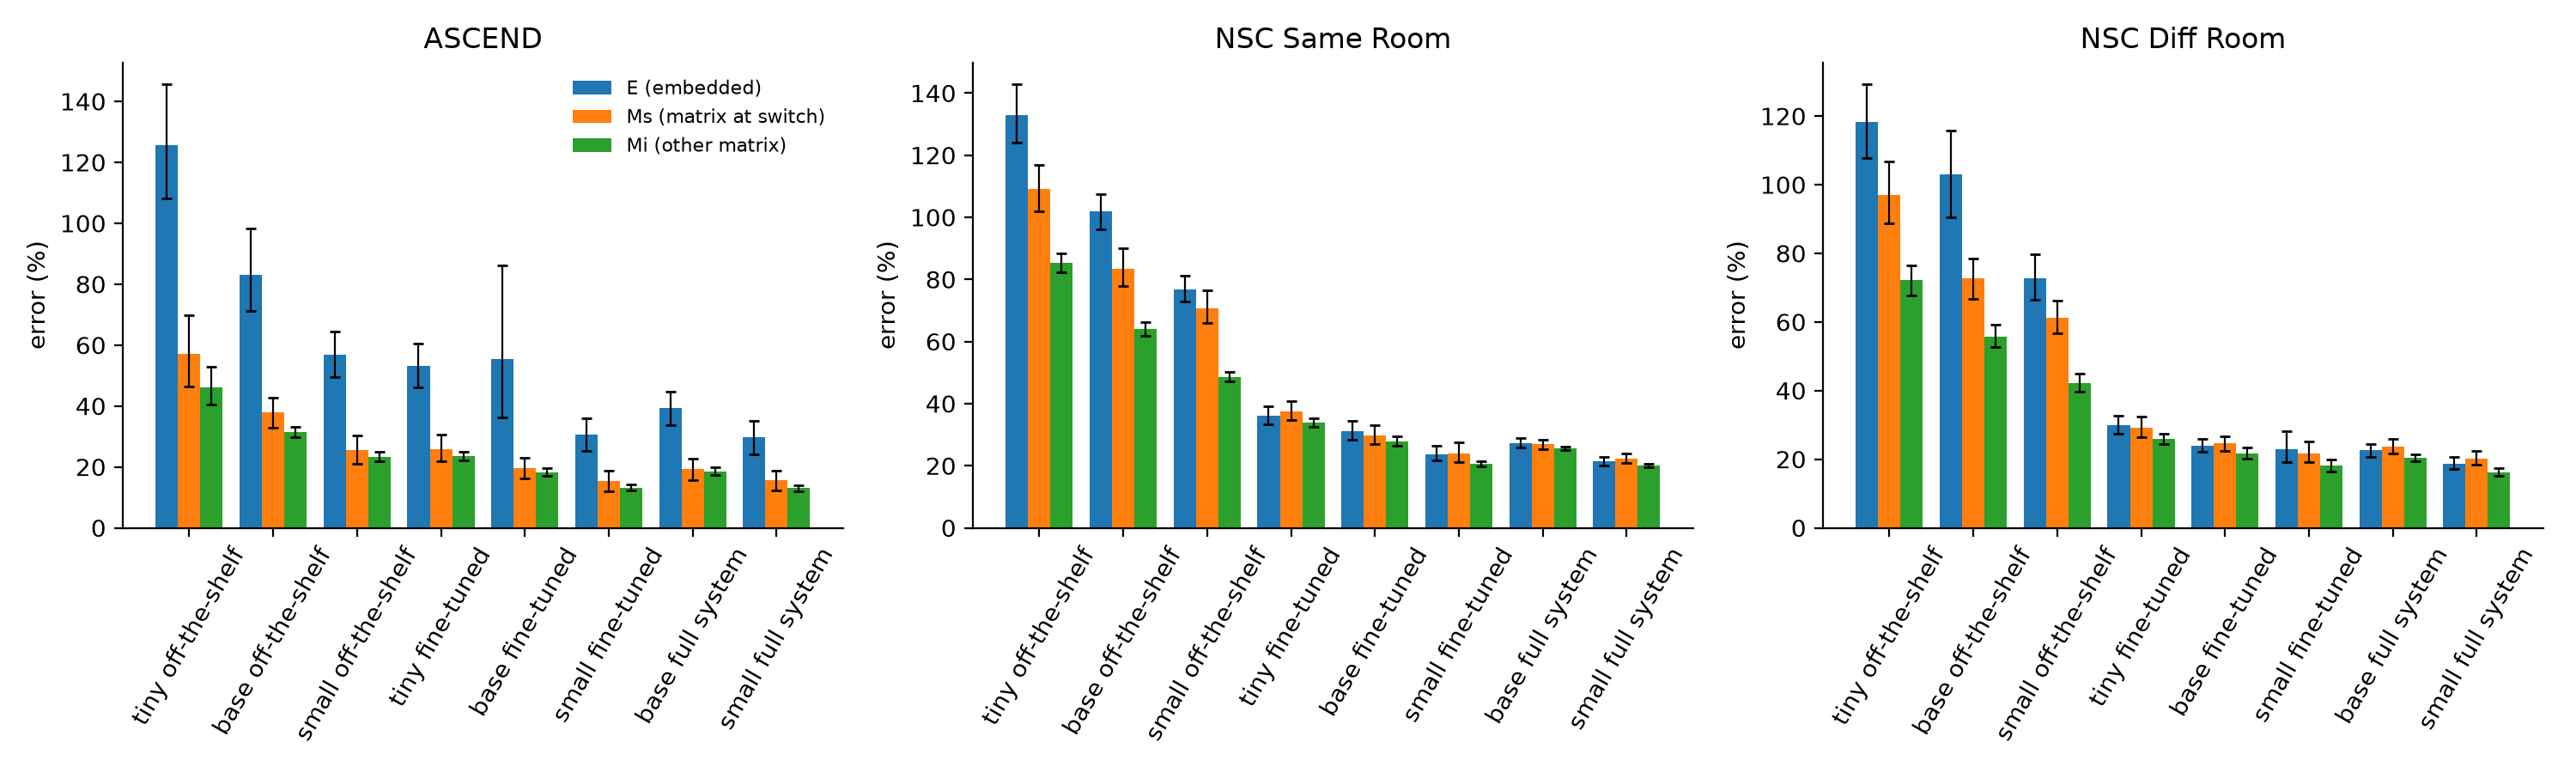
\includegraphics[width=0.9\textwidth]{fig2_role_errors.png}
  \caption{Error rate by role (\Emb, \Ms, \Mi) for each system on the three test sets. Embedded units have the highest error in almost every system.}
  \label{fig:roles}
\end{figure*}



\paragraph{Embedded units fail most.}
In almost every system and test set, embedded units have the highest error, followed by matrix units at a switch and then other matrix units (Figure~\ref{fig:roles}). For off-the-shelf small, embedded error is 56.8\% on ASCEND against 23.4\% for \Mi, and 76.7\% on NSC against 48.6\%.

\begin{table}[t]
\centering
\small
\setlength{\tabcolsep}{3pt}
\resizebox{\columnwidth}{!}{%
\begin{tabular}{lcccc}
\toprule
 & \multicolumn{2}{c}{Same word: \Emb{} $-$ matrix} & \multicolumn{2}{c}{Log-odds} \\
\cmidrule(lr){2-3}\cmidrule(lr){4-5}
System & English & Chinese & $b_{\text{emb}}$ & $b_{\text{emb}\times\text{en}}$ \\
\midrule
small, off-shelf & \textbf{+15.4} & \textbf{+26.0} & \textbf{0.94} & 0.09 \\
base, off-shelf & \textbf{+19.7} & \textbf{+32.0} & \textbf{1.18} & 0.23 \\
base, fine-tuned & \textbf{+8.0} & \textbf{+1.3} & 0.01 & \textbf{0.65} \\
small, fine-tuned & \textbf{+7.4} & +0.3 & $-$0.07 & \textbf{0.79} \\
\bottomrule
\end{tabular}}
\caption{Role vs.\ language. Left: error (points) on the same word type when embedded minus when in the matrix language. Right: logistic-regression coefficients (\S\ref{sec:rq1}). Bold: 95\% CI excludes 0.}
\label{tab:rq1}
\end{table}

\paragraph{The same word is harder when embedded.}
Table~\ref{tab:rq1} (left) compares each word type that occurs in both roles. For off-the-shelf small, an English word is 15.4 points [12.1, 18.6] more likely to be wrong when it is embedded than when it is part of an English-main sentence, and a Chinese character 26.0 points [23.9, 27.8] more. After fine-tuning, the gap for Chinese characters disappears (+0.3 for small) but the gap for English words remains (+7.4 [5.2, 10.1]).

To separate role from language, we fit a logistic regression on 46{,}916 units from 122 speakers:
\begin{equation}
\begin{split}
  \operatorname{logit} P(\text{err}) = {}& b_0 + b_{\text{emb}}\,\text{emb} + b_{\text{en}}\,\text{en} \\
  &+ b_{\text{emb}\times\text{en}}\,\text{emb}\cdot\text{en} \\
  &+ b_f \log f + b_d\, d + b_c\, \text{nsc},
\end{split}
\end{equation}
where emb, en and nsc are 1 if the unit is embedded, is English, or comes from NSC; $f$ is its training-data frequency and $d$ its spoken duration; CIs come from a speaker bootstrap.
Off the shelf, being embedded adds about one unit of log-odds over and above the unit's language ($b_{\text{emb}} = 0.94$ [0.78, 1.15] for small). After fine-tuning, $b_{\text{emb}}$ is about zero, so embedded Mandarin is no longer penalised, but the interaction for embedded English stays large ($0.79$ [0.42, 1.11] for small). \textbf{Fine-tuning removes the role penalty for embedded Mandarin but not for embedded English.}

\paragraph{Errors are transliterations, not translations.}
We expected many embedded errors to be translations. They are not: only 0.5--1.9\% of embedded units are replaced by a translation in the fine-tuned systems (3.4--4.0\% off the shelf). Far more often, the embedded English word is written as Chinese characters that sound like it (deadline$\rightarrow$\zh{得来}, python$\rightarrow$\zh{派森}). This affects up to 10.9\% of embedded units (off-the-shelf small on NSC 10.7\%; full small 2.5--3.8\%). The conclusion holds for every translation threshold $\tau \le 0.7$ (Appendix~\ref{sec:appendix}). A human audit of 30 random pairs confirms that translations are rare (none among the 26 labelled), but it labels most of the pairs our labels call transliterations as unrelated (\S\ref{sec:limitations}), so the transliteration rates are best read as upper bounds.
